% !TEX root = ../main.tex
\subsection{Results}
% !TEX root = ../main.tex
\begin{table}[t]
    \centering
    \begin{tabular}{l|c|c}
    Models                             & Acc.                  & Acc.  w/ D              \\
    \hline\hline
    Supervised                         & 94.62 $\pm$ 0.09      & 94.62 $\pm$ 0.09        \\
    \hline
    Semi-Supervised Inference          & 97.45 $\pm$ 0.05      & 95.08 $\pm$ 0.09        \\
    \hline\hline
    Soft $k$-Means                     & 97.25 $\pm$ 0.10      & 95.01 $\pm$ 0.09        \\
    \hline
    Soft $k$-Means+Cluster             & \tb{97.68 $\pm$ 0.07} & 97.17 $\pm$ 0.04        \\
    \hline
    Masked Soft $k$-Means              & 97.52 $\pm$ 0.07      & \tb{97.30 $\pm$ 0.08}   \\
    \end{tabular}
    \caption{Omniglot 1-shot classification results. ``w/ D'' denotes ``with distractors'' where the
    unlabeled images contain irrelevant classes.}
    \label{tab:omniglot}
\end{table}

% !TEX root = ../main.tex
\begin{table}[t]
    \centering
    \resizebox{\textwidth}{!}{
    \begin{tabular}{l|c|c|c|c}
    Models                       & 1-shot Acc.         & 5-shot Acc.         & 1-shot Acc w/ D     & 5-shot Acc. w/ D \\
    \hline\hline
    Supervised                   & 43.61 $\pm$ 0.27    & 59.08 $\pm$ 0.22   & 43.61 $\pm$ 0.27    & 59.08 $\pm$ 0.22 \\
    \hline
    Semi-Supervised Inference    & 48.98 $\pm$ 0.34    & 63.77 $\pm$ 0.20    & 47.42 $\pm$ 0.33    & 62.62 $\pm$ 0.24 \\
    \hline\hline
    Soft $k$-Means               &\tb{50.09 $\pm$ 0.45}&\tb{64.59 $\pm$ 0.28}&\tb{48.70 $\pm$ 0.32}&\tb{63.55 $\pm$ 0.28}\\
    \hline
    Soft $k$-Means+Cluster       & 49.03 $\pm$ 0.24    & 63.08 $\pm$ 0.18    &\tb{48.86 $\pm$ 0.32}& 61.27 $\pm$ 0.24 \\
    \hline
    Masked Soft $k$-Means        &\tb{50.41 $\pm$ 0.31}&\tb{64.39 $\pm$ 0.24}&\tb{49.04 $\pm$ 0.31}& 62.96 $\pm$ 0.14 \\
    \end{tabular}
    }
    \caption{{\it mini}ImageNet 1/5-shot classification results. ``w/ D'' denotes ``with
    distractors'' where the unlabeled images contain irrelevant classes.}
    \label{tab:miniImageNet}
\end{table}

% !TEX root = ../main.tex
\begin{table}[t]
    \centering
    \resizebox{\textwidth}{!}{
    \begin{tabular}{l|c|c|c|c}
    Models                    & 1-shot Acc.         & 5-shot Acc.         & 1-shot Acc. w/ D    & 5-shot Acc. w/ D     \\
    \hline\hline
    Supervised                & 46.52 $\pm$ 0.52    & 66.15 $\pm$ 0.22    & 46.52 $\pm$ 0.52    & 66.15 $\pm$ 0.22     \\
    \hline
    Semi-Supervised Inference & 50.74 $\pm$ 0.75    & 69.37 $\pm$ 0.26    & 48.67 $\pm$ 0.60    & 67.46 $\pm$ 0.24      \\
    \hline\hline
    Soft $k$-Means            & 51.52 $\pm$ 0.36    &\tb{70.25 $\pm$ 0.31}& 49.88 $\pm$ 0.52    & 68.32 $\pm$ 0.22     \\
    \hline
    Soft $k$-Means+Cluster    &\tb{51.85 $\pm$ 0.25}& 69.42 $\pm$ 0.17    &\tb{51.36 $\pm$ 0.31}& 67.56 $\pm$ 0.10     \\
    \hline
    Masked Soft $k$-Means     &\tb{52.39 $\pm$ 0.44}&\tb{69.88 $\pm$ 0.20}&\tb{51.38 $\pm$ 0.38}&\tb{69.08 $\pm$ 0.25} \\
    \end{tabular}
    }
    \caption{\textit{tiered}ImageNet 1/5-shot classification results. ``w/ D'' denotes ``with
    distractors'' where the unlabeled images contain irrelevant classes.}
    \label{tab:tieredImageNet}
\end{table}
\begin{figure}
    \centering
    \iflatexml
    \includegraphics[width=\textwidth]{figures/tnet_num_unlabel.png}
    \else
    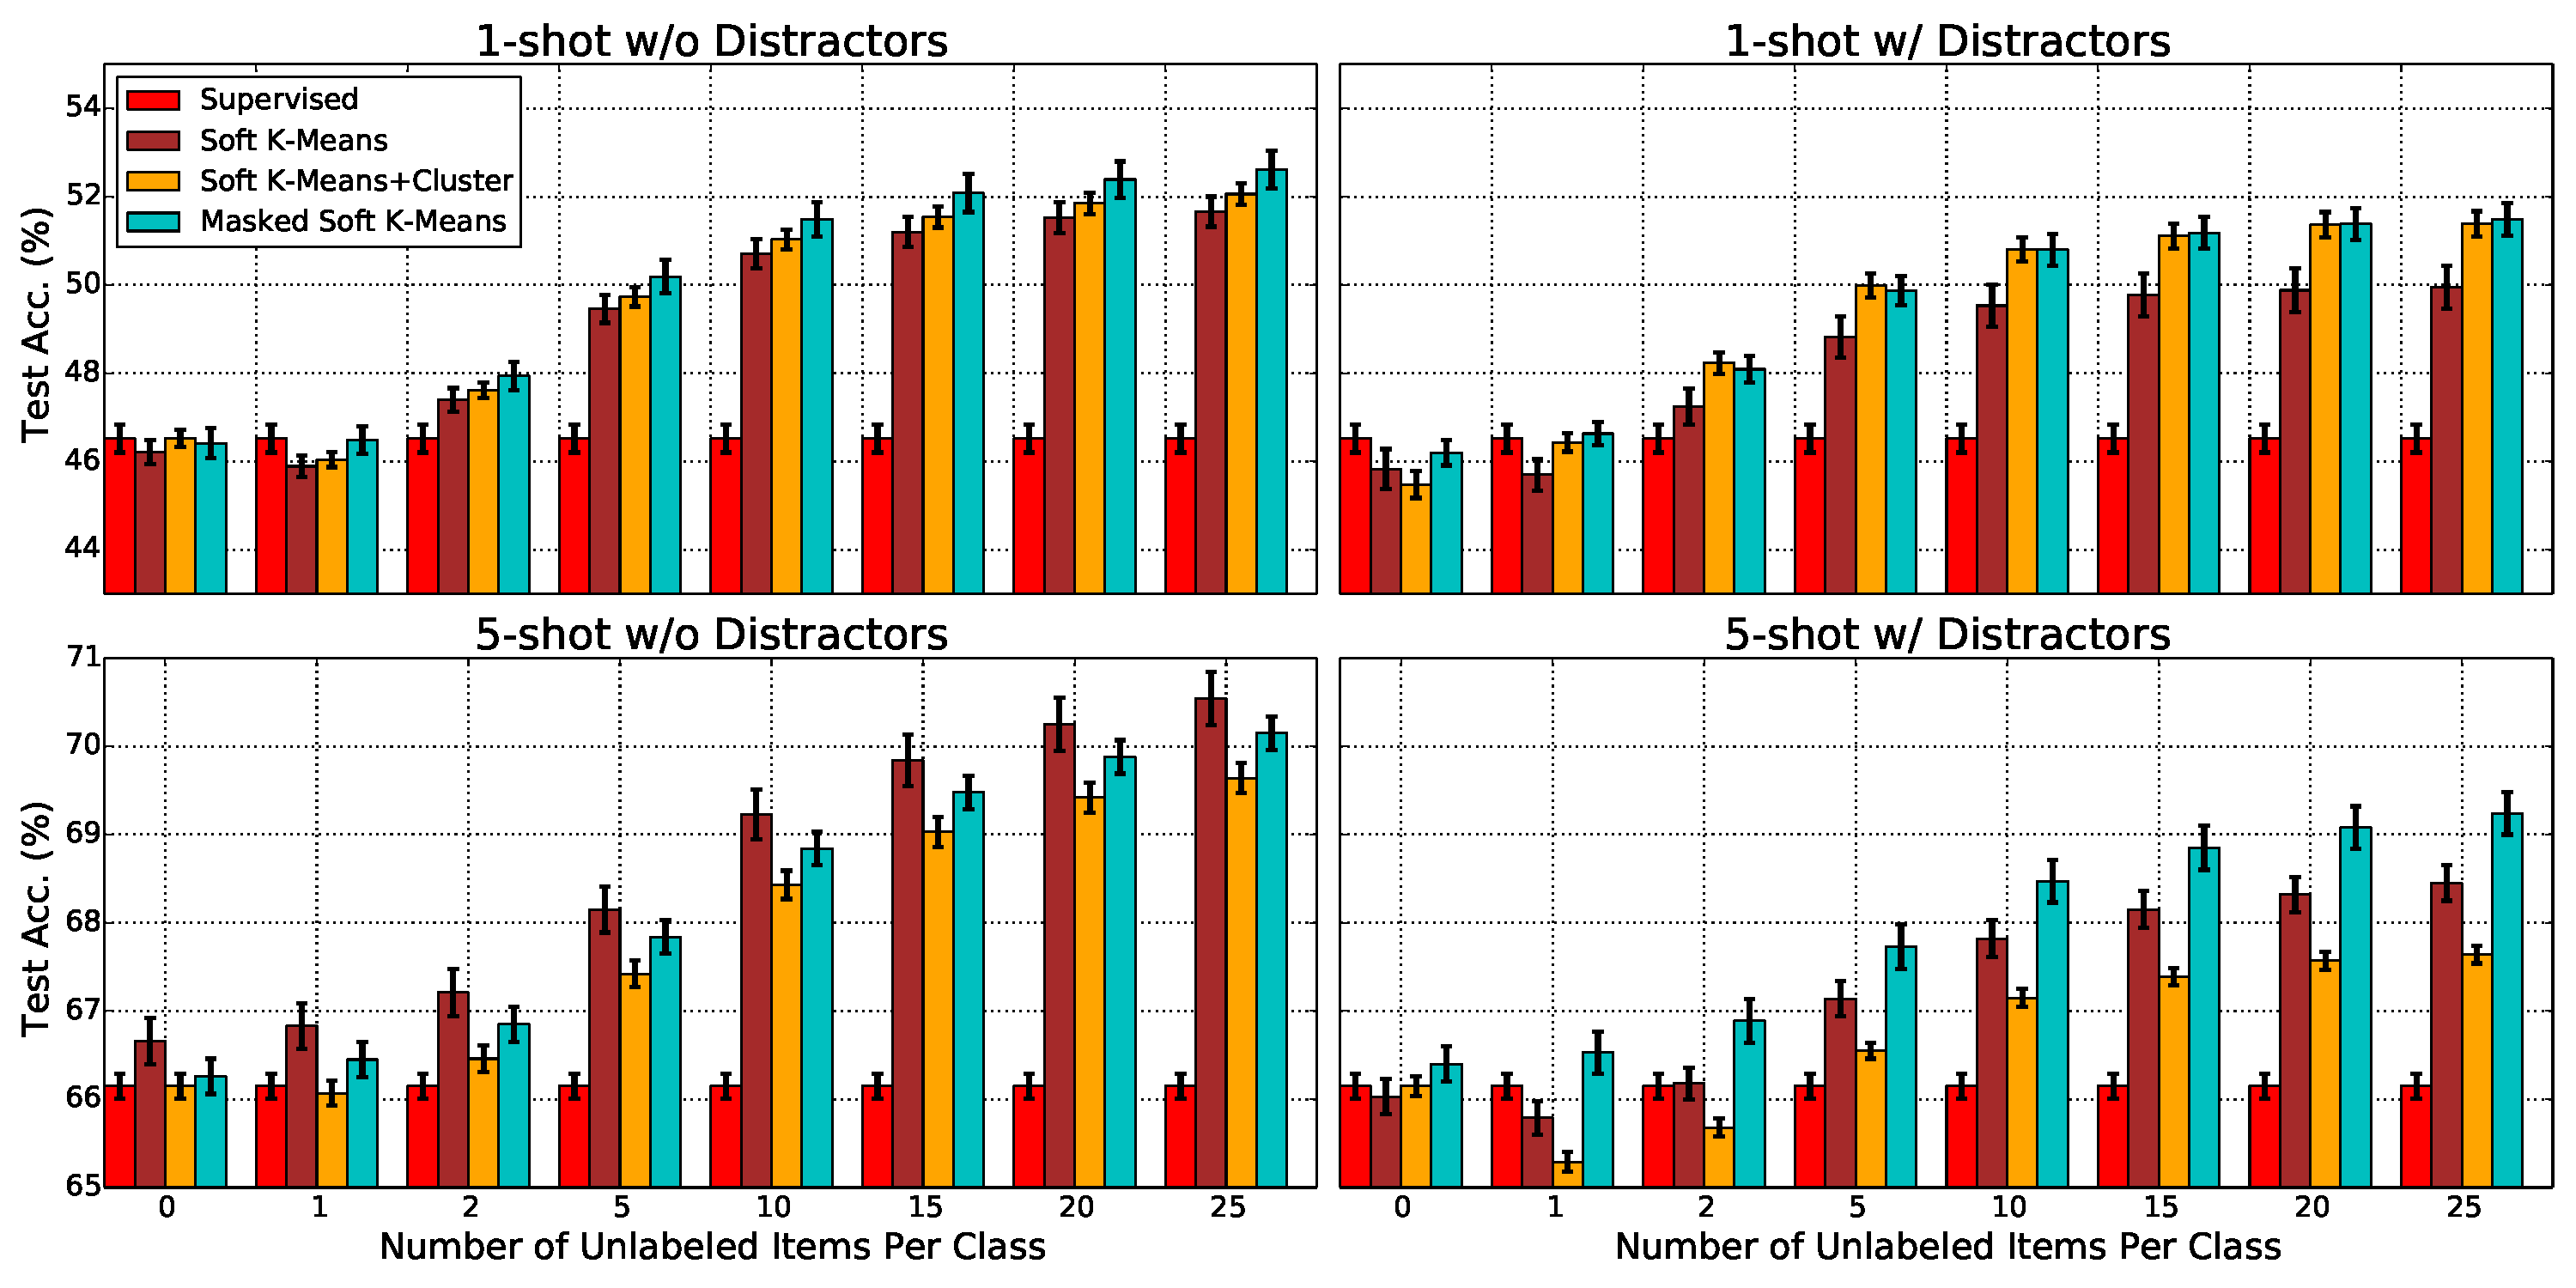
\includegraphics[width=\textwidth]{figures/tnet_num_unlabel.pdf}
    \fi
    \caption{Model Performance on {\it tiered}ImageNet with different number of unlabeled items during test time.}
    \label{fig:tnet_num_unlabel}
\end{figure}

Results for Omniglot, {\it mini}ImageNet and {\it tiered}ImageNet are given in
Tables~\ref{tab:omniglot},~\ref{tab:miniImageNet} and~\ref{tab:tieredImageNet}, respectively, while
Figure~\ref{fig:tnet_num_unlabel} shows the performance of our models on {\it tiered}ImageNet (our
largest dataset) using different values for $M$ (number of items in the unlabeled set per class).

Across all three benchmarks, at least one of our proposed models outperform the baselines,
demonstrating the effectiveness of our semi-supervised meta-learning procedure. 
In particular, 
both
Soft $k$-Means and Soft $k$-Means+Cluster perform well on 1-shot non-distractor settings, and 
Soft $k$-Means is better on 5-shot, as it considers the most unlabeled examples. 
With the presence of distractors, Masked Soft $k$-Means shows the most robust performance across all
three datasets, reaching comparable performance compared to the upper bound of the best under
non-distractor settings.

% For 5-shot, Masked soft $k$-Means reaches comparable performance compared to the upper bound
% of the best non-distractor performance.

From Figure~\ref{fig:tnet_num_unlabel}, we observe clear improvement in test accuracy when the
number grows from 0 to 25. Note that our models were trained with $M=5$ and thus are showing an
ability to extrapolate in generalization. This confirms that, through meta-training, the models
learned to acquire a better representation that will be more helpful after semi-supervised
refinement.

Note that the wins obtained in our semi-supervised learning are super-additive. Consider the case of
the simple $k$-Means model on 1-shot without Distractors. Training only on labeled examples while
incorporating the unlabeled set during test time produces an advantage of 4.2\% (50.7-46.5), and
incorporating unlabeled examples during both training and test yields a win of 5.9\% (52.4-46.5).
